\documentclass[letterpaper, oneside]{book}

\usepackage{tree-dvips}
\usepackage{amsmath}
\usepackage{amsthm}
\usepackage{listings}
\usepackage{graphicx}
\usepackage{xcolor}
\usepackage{mdframed}
\usepackage{fancyhdr}
\usepackage[export]{adjustbox}
\usepackage[skip=10pt]{parskip}
\usepackage{amsfonts}
\usepackage{hyperref}
\usepackage{algorithm}
\usepackage{algpseudocode}
\pagestyle{plain}
\usepackage{enumitem}

\setlist{nolistsep}
\setlist[itemize]{topsep=0em, itemsep=0.2em, label={$\bullet$}}

% Configure listings backage for code
\lstset{
    %numbers=left,
    %numberstyle=\tiny,
    breaklines=true,
    %numbersep=5pt,
    xleftmargin=.45in,
    xrightmargin=.05in}

\graphicspath{{./resources/}}

\hypersetup{pdfborder=0 0 0}
\theoremstyle{definition}
\newtheorem*{definition}{Definition}

\theoremstyle{remark}
\newtheorem*{remark}{Remark}


\title{System Design Notes}
\author{Ryan}
\date{July 2024}

\begin{document}

\maketitle{}
\tableofcontents


%%%%%%%%%%%%%%%%%%%%%%%%%%%%%%%%%%%%%%%%%%%%%%%%%%%%
%%%%%%%%%%%%%%%%%%%%%%%%%%%%%%%%%%%%%%%%%%%%%%%%%%%%
\part{Warm-up}

%%%%%%%%%%%%%%%%%%%%%%%%%%%%%%%%%%%%%%%%%%%%%%%%%%%%
\chapter{Introduction}
%%%%%%%%%%%%%%%%%%%%%%%%%%%%%%%%%%%%%%%%%%%%%%%%%%%%

test
\begin{itemize}
    \item system coordination
    \item resource management
    \item indexing
    \item remote communication
    \item serialization
\end{itemize}

%%%%%%%%%%%%%%%%%%%%%%%%%%%%%%%%%%%%%%%%%%%%%%%%%%%%
\chapter{Keywords}
%%%%%%%%%%%%%%%%%%%%%%%%%%%%%%%%%%%%%%%%%%%%%%%%%%%%

DNS; monolithic; tiered architecture; database management system; relational database; vertical scaling; horizontal scaling; failover; redundancy; load balancer; database replication; cache; eviction policy; expiration policy; consistent hashing; cache miss; cache hit; caching strategy; single point of failure; stateful webserver; stateless webserver; CDN; message queue; normalization; de-normalization; sharding; rate limiting; optimistic lock; eventual consistency; transaction log; lease; fan-out; rollback; read-your-write

\chapter{Real-life Examples}

\section{Email and News Letter}
\section{Git Version Control}
\section{Calendar App}
\section{Waiting Lines and Queue}
\section{Google Doc}

%%%%%%%%%%%%%%%%%%%%%%%%%%%%%%%%%%%%%%%%%%%%%%%%%%%%
%%%%%%%%%%%%%%%%%%%%%%%%%%%%%%%%%%%%%%%%%%%%%%%%%%%%
\part{Fundamentals and Building Blocks}


%%%%%%%%%%%%%%%%%%%%%%%%%%%%%%%%%%%%%%%%%%%%%%%%%%%%
\chapter{Log}
%%%%%%%%%%%%%%%%%%%%%%%%%%%%%%%%%%%%%%%%%%%%%%%%%%%%

\section{Ordered Sequence of Records}
The term "log" carries a more general meaning than the common use case as the one in the term "application log"

\begin{definition}[Log]
    Log is an append-only sequence of records ordered by time.
\end{definition}

Each entry appended to the log is assigned a unique sequential log entry number that acts as its unique key. The log entry number is ordered and can be thought as the "timestamp" of the entry. In fact, the log entry number defines a logical time.

Logs have a specific purpose: they record what happened and when. They servers as the authoritative source of events history.


It's important to emphasis again that logs have two important properties:
\begin{itemize}
    \item They are ordered records.
    \item Once the records are persisted, they become immutable.
\end{itemize}

These two properties have immediate implications:
\begin{itemize}
    \item The log entry number can be used as an identifier of states.
    \item Thanks to the immutability, logs support replay, which is closely related to recovery. In fact, with logs, we can reconstruct states.
\end{itemize}

Many distributed system problems can be reduced to the handling of logs. For example, consider the task of synchronizing two machines so that their data is consistent. This problem can be reduced to synchronizing logs on these two machines.

\section{Examples}
As a developer, we are all familiar with application logs. Each line in the log file represents an event. There are tools that can monitor log files and if some special events are detected, the tool will send out notifications or alerts. As we can see, logs can be used as the source or producers of events. Another example is the transaction log in the database context. They can be monitored and used to trigger data change events.

TODO: log shipping protocol

%%%%%%%%%%%%%%%%%%%%%%%%%%%%%%%%%%%%%%%%%%%%%%%%%%%%
\chapter{Consistent Hashing}
%%%%%%%%%%%%%%%%%%%%%%%%%%%%%%%%%%%%%%%%%%%%%%%%%%%%
\begin{definition}[Consistent Hashing]
    test
\end{definition}

%%%%%%%%%%%%%%%%%%%%%%%%%%%%%%%%%%%%%%%%%%%%%%%%%%%%
\chapter{Cache}
%%%%%%%%%%%%%%%%%%%%%%%%%%%%%%%%%%%%%%%%%%%%%%%%%%%%

caching strategy; expiration policy; eviction policy; invalidation

Caches and cache layers are key components in almost every high-performance architecture. The idea is to save results that are expensive to obtain. Examples are prediction calculated by a complex machine learning algorithms or data extracted from a database.

When employing caches, it's important to remember two important characteristics of caches:
\begin{itemize}
    \item It requires additional efforts to maintain the consistency between caches and the authoritative source of the data.
    \item Caches are ephemeral. When designing a system that uses caches, we need to assume we could lose the cached items at anytime.
\end{itemize}


\begin{itemize}
    \item expiration policy
    \item eviction policy
    \item invalidation
    \item marker
    \item partition vs replication
    \item pool and region
\end{itemize}


Difference between partition and replication

As shown in the figure \ref{fig:partition_vs_replication}

\begin{figure}[h]
    \centering
    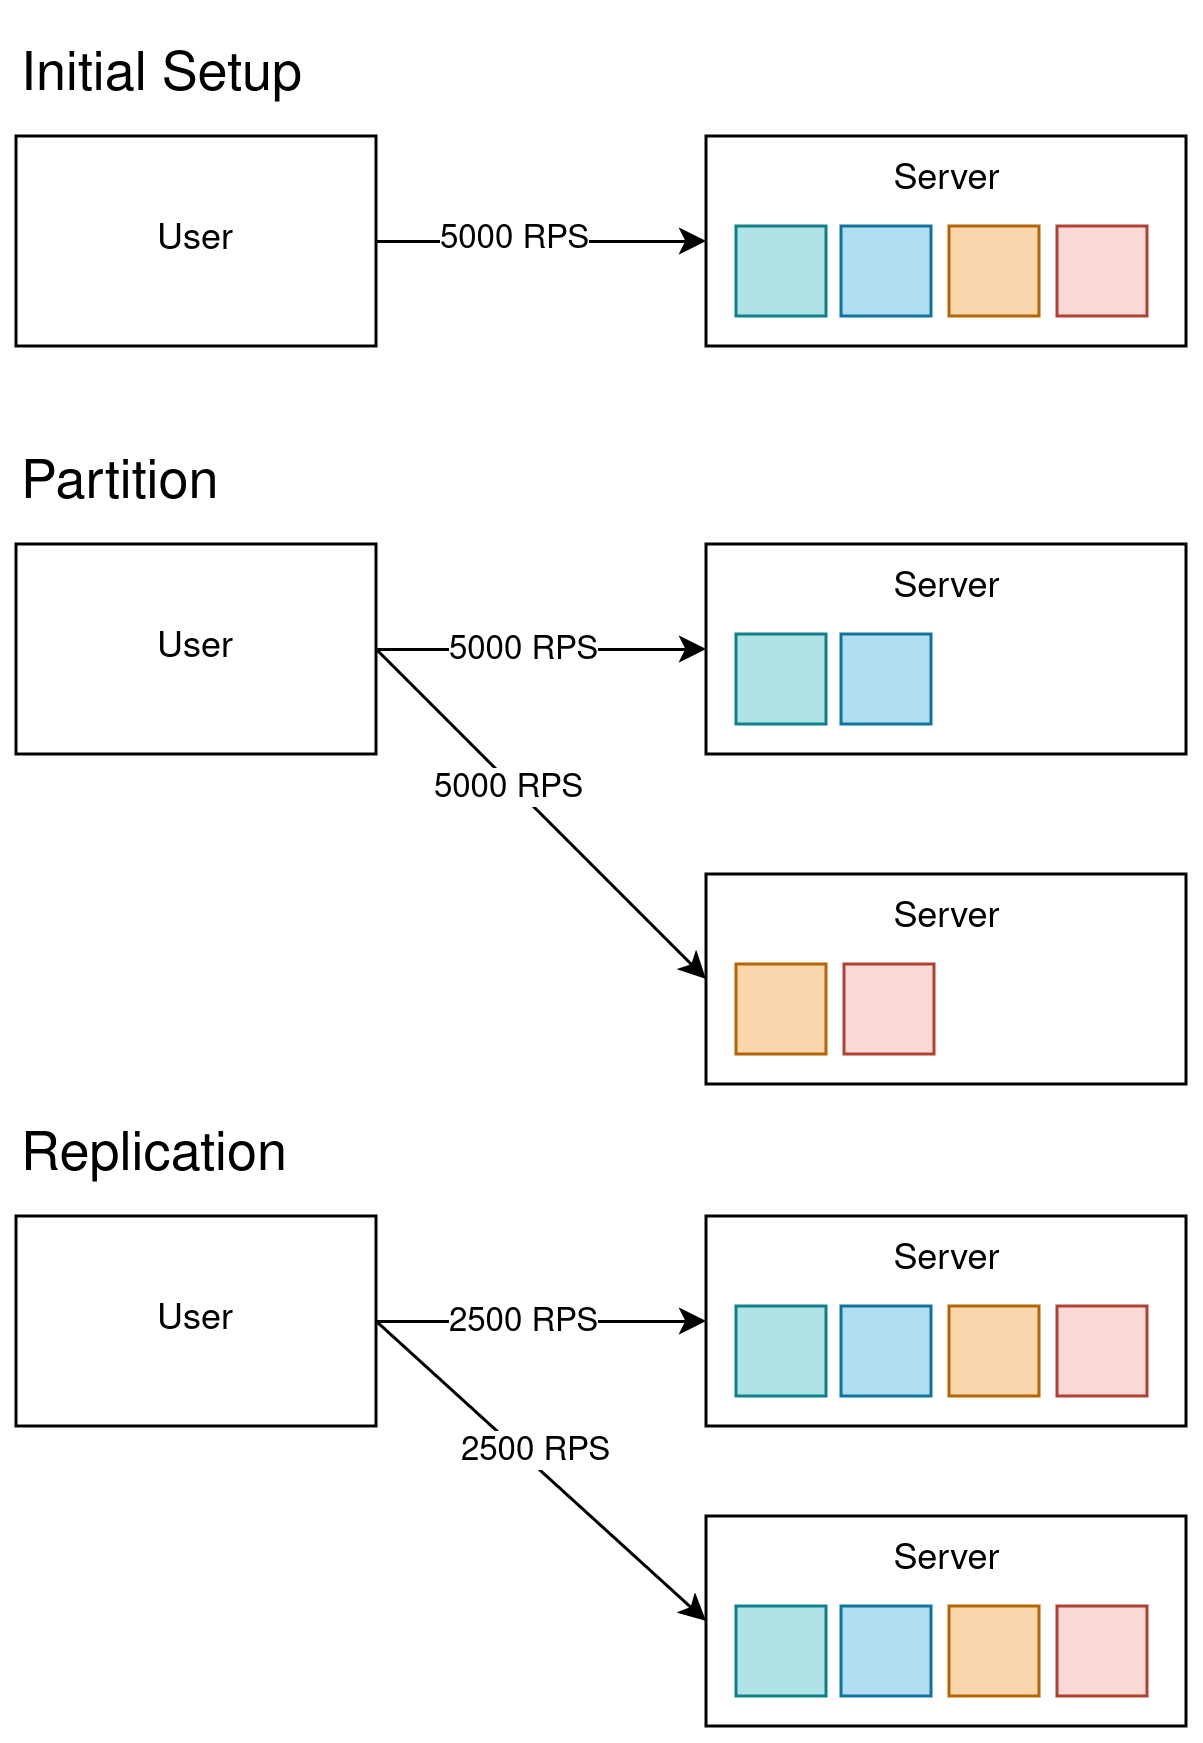
\includegraphics[height=0.60\textwidth]{partition_vs_replication.png}
    \caption{Partition vs replication}
    \label{fig:partition_vs_replication}
\end{figure}


\section{Distributed Cache}


%%%%%%%%%%%%%%%%%%%%%%%%%%%%%%%%%%%%%%%%%%%%%%%%%%%%
\chapter{Lock}
%%%%%%%%%%%%%%%%%%%%%%%%%%%%%%%%%%%%%%%%%%%%%%%%%%%%

\subsection{Default Locking}

\subsection{Optimistic Locking}

\subsection{Distributed Locks}

%%%%%%%%%%%%%%%%%%%%%%%%%%%%%%%%%%%%%%%%%%%%%%%%%%%%
\chapter{Message Queue}
%%%%%%%%%%%%%%%%%%%%%%%%%%%%%%%%%%%%%%%%%%%%%%%%%%%%


%%%%%%%%%%%%%%%%%%%%%%%%%%%%%%%%%%%%%%%%%%%%%%%%%%%%
\chapter{Design Patterns}
%%%%%%%%%%%%%%%%%%%%%%%%%%%%%%%%%%%%%%%%%%%%%%%%%%%%

\section{Partition}
Partition or sharding is a direct application of the divide-and-conquer strategy. Instead of routing all the work to a single machine, we distribute the work to a cluster of machines. Partitioning the workload is a crutial step if we want to horizontally scale the system. The partitioning implementation needs to take into account the fact the size of cluster may change.

For example, during a cluster maintenance, some machines may be shutdown, resulting in a decrease of the cluster capacity. Or we may need to add more machines to accommodate an increase in the request load. When the cluster size changes, requests may be routed to a different machines, which may not be ready to process the request efficiently. A typical solution to this problem is consistent hashing.


\section{Leader Follower Pattern}

\section{Quorum}

\begin{displaymath}
    W + R > N
\end{displaymath}

\section{Batch}

This can happen in many places:
\begin{itemize}
    \item form client to server when sending data
    \item in writes to disk
    \item in replication between servers
    \item in data transfer to consumers
    \item in acknowledging committed data
\end{itemize}

The main idea is to reduce the number of network round trips.



%%%%%%%%%%%%%%%%%%%%%%%%%%%%%%%%%%%%%%%%%%%%%%%%%%%%
\chapter{Classic Architecture}
%%%%%%%%%%%%%%%%%%%%%%%%%%%%%%%%%%%%%%%%%%%%%%%%%%%%

\section{Basic Template}

The diagram below demonstrates one of the basic structures of application services. Uses, such as mobile devices or applications running on servers send request to the endpoint of the target services. When the user request enters the service boundary, it usually hits a load balancer first. The load balancer is responsible for evenly distribute use requests to application servers in the cluster. The

For application servers form a cluster, there is usually a piece of code responsible for coordination. Servers may play different roles in a cluster, for example, some of the servers are coordinators and others are workers.



\begin{figure}[h]
    \centering
    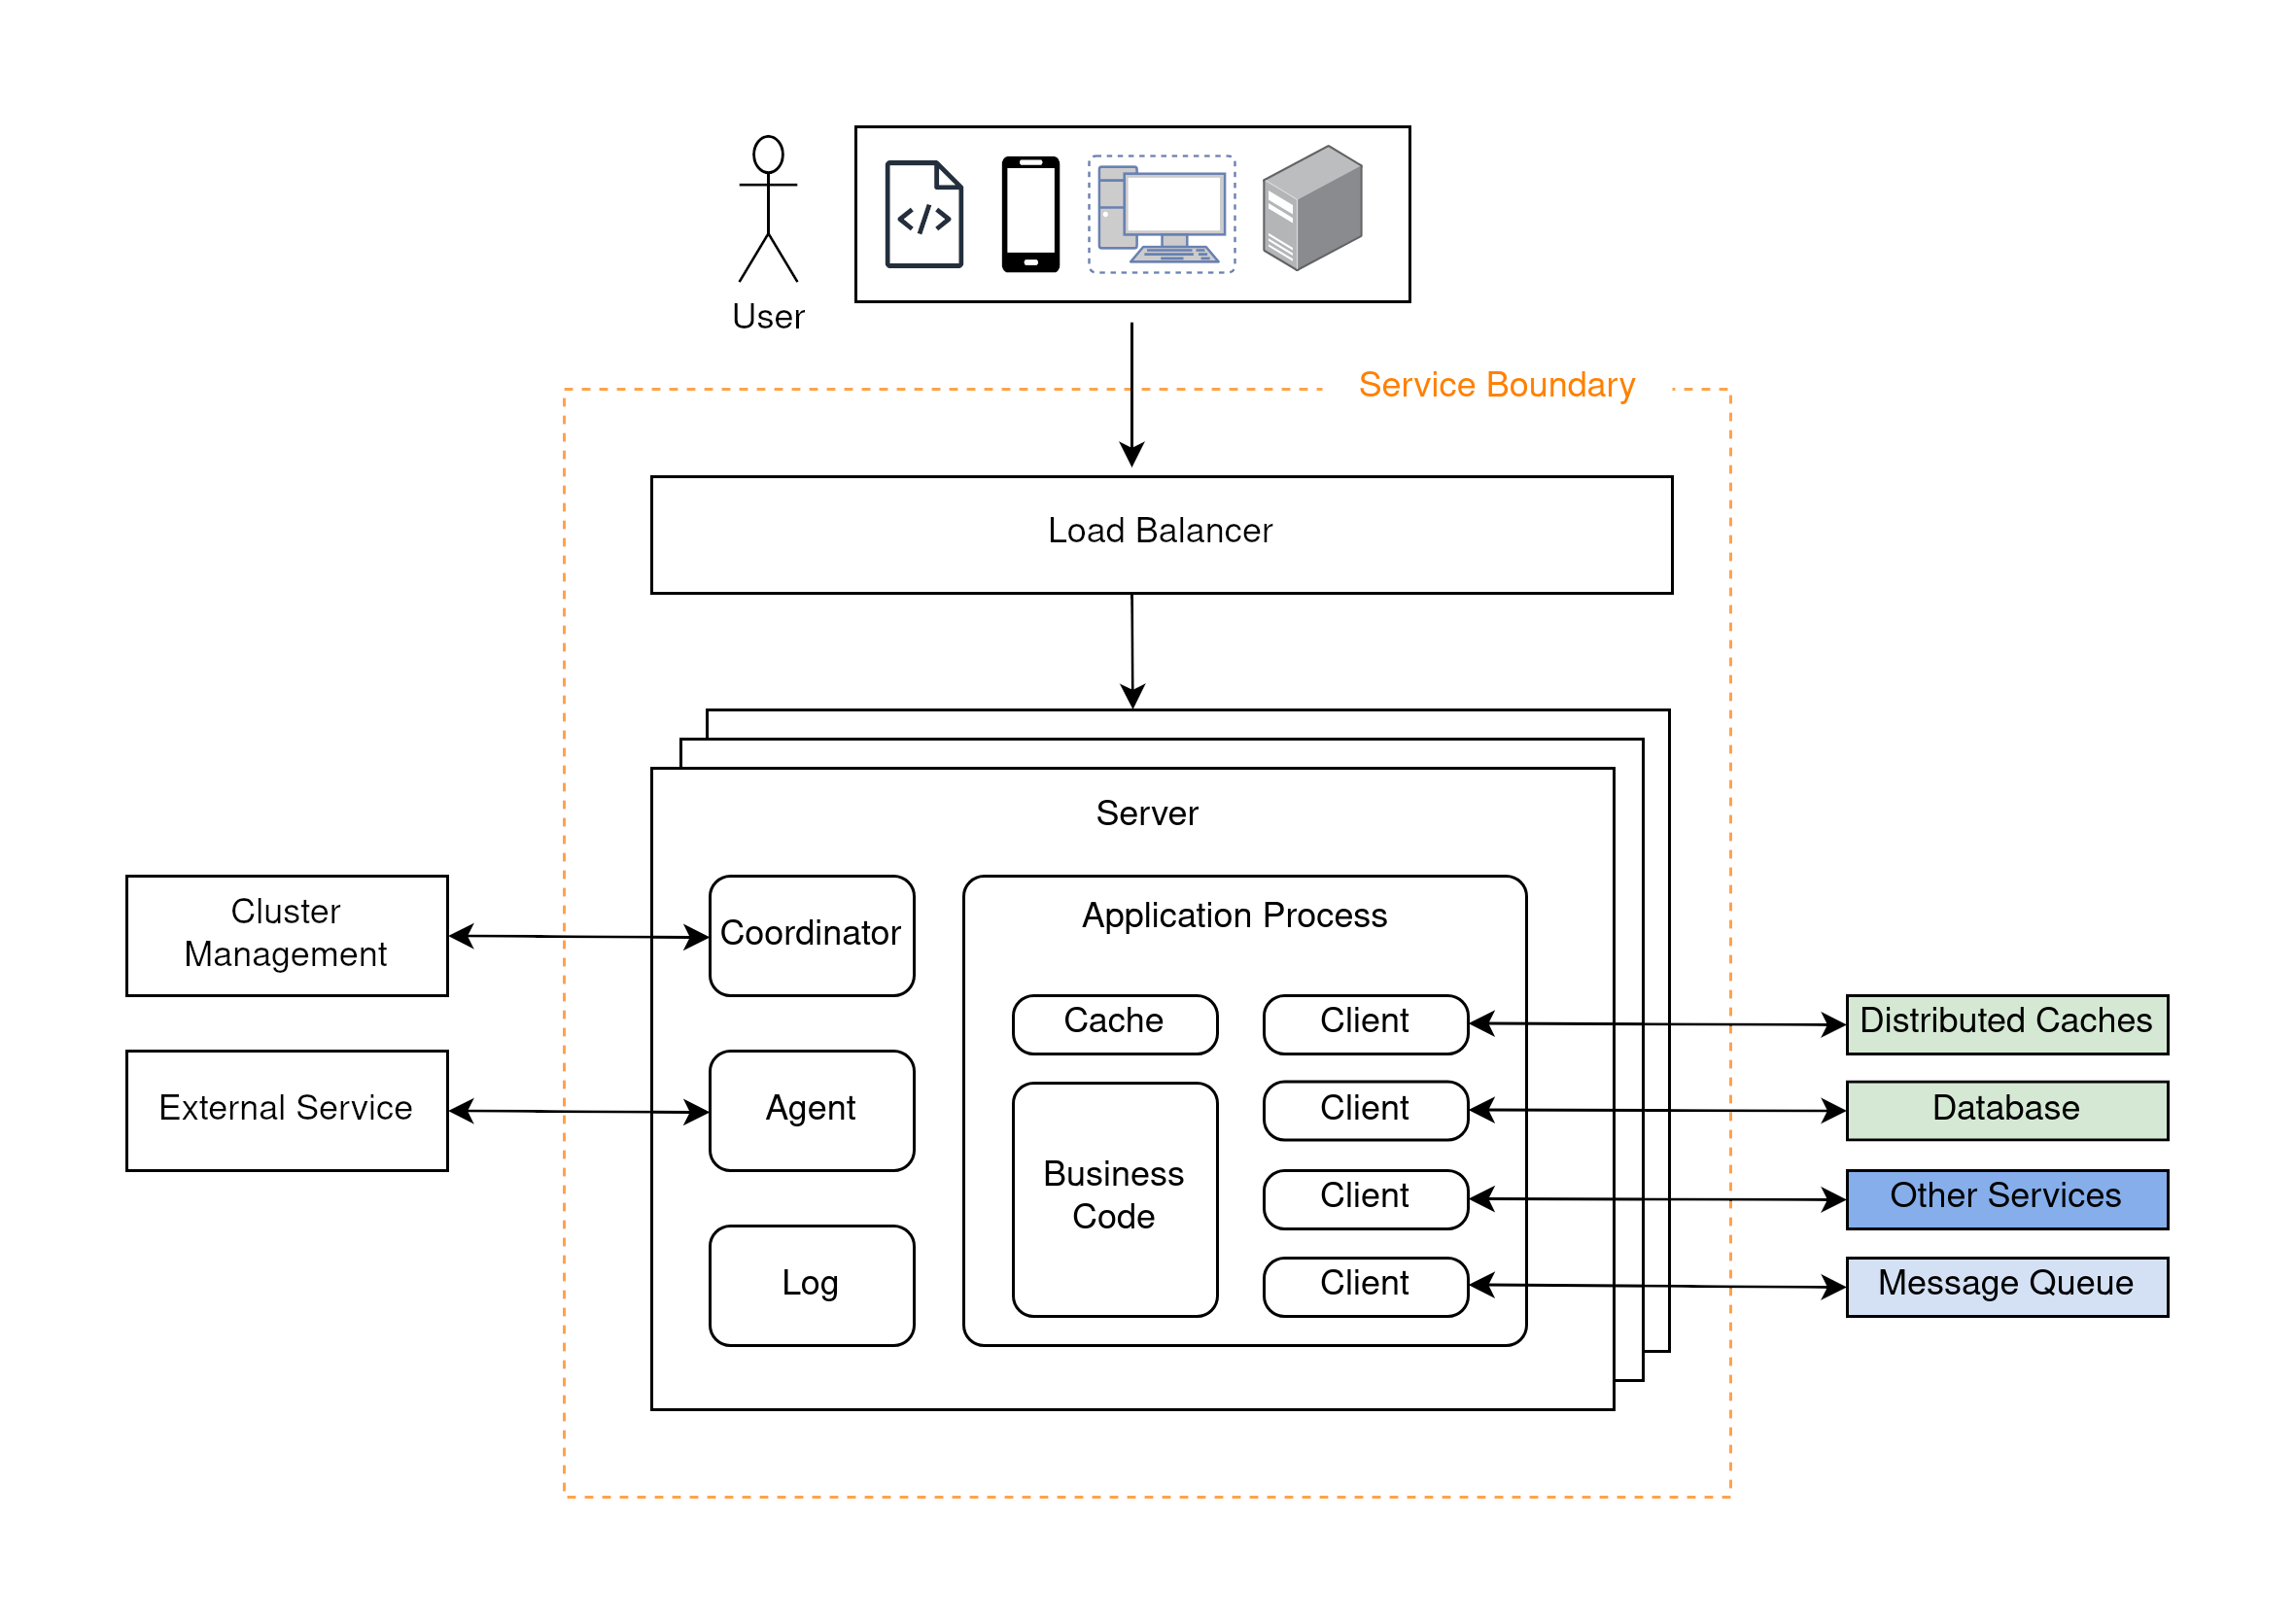
\includegraphics[width=0.90\textwidth]{system_design_basic_template.png}
    \caption{A basic template}
    \label{fig:basic_template}
\end{figure}


%%%%%%%%%%%%%%%%%%%%%%%%%%%%%%%%%%%%%%%%%%%%%%%%%%%%
\chapter{Data Modeling}
%%%%%%%%%%%%%%%%%%%%%%%%%%%%%%%%%%%%%%%%%%%%%%%%%%%%
normalization; denormalization


%%%%%%%%%%%%%%%%%%%%%%%%%%%%%%%%%%%%%%%%%%%%%%%%%%%%
%%%%%%%%%%%%%%%%%%%%%%%%%%%%%%%%%%%%%%%%%%%%%%%%%%%%
\part{Cloud Technology}

%%%%%%%%%%%%%%%%%%%%%%%%%%%%%%%%%%%%%%%%%%%%%%%%%%%%
\chapter{AWS}
%%%%%%%%%%%%%%%%%%%%%%%%%%%%%%%%%%%%%%%%%%%%%%%%%%%%


\part{Database}

%%%%%%%%%%%%%%%%%%%%%%%%%%%%%%%%%%%%%%%%%%%%%%%%%%%%
\chapter{Relational Database}
%%%%%%%%%%%%%%%%%%%%%%%%%%%%%%%%%%%%%%%%%%%%%%%%%%%%
transaction log; commit log;


%%%%%%%%%%%%%%%%%%%%%%%%%%%%%%%%%%%%%%%%%%%%%%%%%%%%
\chapter{Non-relational Database}
%%%%%%%%%%%%%%%%%%%%%%%%%%%%%%%%%%%%%%%%%%%%%%%%%%%%

Non-relational databases might be the right choice if:
\begin{itemize}
    \item Your application requires super-low latency.
    \item Your data are unstructured, or you do not have any relational data.
    \item You only need to serialize and deserialize data.
    \item You need to store a massive amount of data.
\end{itemize}






\end{document}
